\documentclass[a4paper, 11pt]{article}

\usepackage[portuges]{babel}
\usepackage[utf8]{inputenc}
\usepackage{amsmath}
\usepackage{indentfirst}
\usepackage[table,xcdraw]{xcolor}
\usepackage{graphicx}
\usepackage{tabto}
\usepackage{float}
\usepackage{adjustbox}
\usepackage[pdftex]{color,graphicx}
\usepackage[left=2cm,top=2.5cm,right=2.5cm,bottom=2.5cm]{geometry}
\usepackage{enumerate}% http://ctan.org/pkg/enumerate
\usepackage{xurl}
\usepackage{hyperref}

\begin{document}
\begin{titlepage}
    \begin{center}

    	
\includegraphics[width=0.3\textwidth]{images/Capa/EEUMfinal .png}
       
       \vspace*{1cm}
       
       \textbf{\Large Engenharia de Serviços em Rede}
        \vspace{1cm}
        \par
        \textbf{\Large Nível Aplicacional: Conceitos Introdutórios }
        \vspace{1cm}
        \par
        \Large \textbf{PL3 - Grupo 5}
        
       Luis Sousa a89597\\Maria Barros pg47488\\Pedro Barbosa pg47577
       \vspace{1cm}
	\begin{figure}[!htb]
	    \hspace{1.5cm}
        \minipage{0.25\textwidth}%
            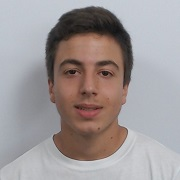
\includegraphics[width=\linewidth]{images/Capa/80.jpg} 
            \centering
            \captionsetup{a89597}
        \endminipage
        \hspace{-0.2cm}
        \minipage{0.25\textwidth}%
            
\includegraphics[width=\linewidth]{images/Capa/44.jpg} 
            \centering
            \captionsetup{pg47488}
        \endminipage
        \hspace{-0.2cm}
        \minipage{0.25\textwidth}%
            
\includegraphics[width=\linewidth]{images/Capa/154.jpg} 
            \centering
            \captionsetup{pg47577}
        \endminipage
    \end{figure}

\blindtext

\vspace{2cm}
        
        26 de outubro de 2020
            
    \end{center}
\end{titlepage}

\newpage
\tableofcontents
\newpage
\section {Questão 1} 
\textbf{As aplicações em rede assentam normalmente em paradigmas cliente-servidor ou peer-to-peer.}
\subsection{Alinea a} 
\textbf{Explique em que se diferenciam ambos os modelos, salientando o papel das principais entidades envolvidas.}

\vspace{0.5cm}

A principal diferença entre os paradigmas cliente-servidor e \textit{peer-to-peer} é que, no primeiro, a gestão de dados é centralizada enquanto que no segundo modelo cada utilizador tem as suas próprias aplicações e dados, sendo a gestão destes últimos distribuída.

No que concerne ao papel das principais entidades envolvidas no modelo cliente-servidor existe a distinção entre clientes que fazem pedidos de serviços e servidores que respondem com o serviço pedido. Neste, os servidores têm um endereço \textit{IP} permanente e funcionam como bases de dados para efeitos de escalabilidade enquanto os clientes possuem endereços \textit{IP} dinâmicos, podem estar conectados intermitentemente e apenas comunicam com o servidor e nunca entre si mesmos. No paradigma \textit{peer-to-peer}, cada nodo está conectado intermitentemente e tem a capacidade de mudar o seu endereço \textit{IP}, pedir serviços e providenciar os mesmos, funcionando como cliente ou como servidor, tornando a sua gestão complexa. Desta forma, este modelo acaba por ter uma escalabilidade própria, na medida em que a criação de novos nodos desenvolve uma maior capacidade de serviço e, consequentemente, uma maior quantidade de pedidos de serviço. \cite{1_a}


\subsection{Alinea b \cite{1_b1, 1_b2, 1_b3, 1_b4, 1_b5}} 
\textbf{Enuncie vantagens e desvantagens de cada paradigma e casos de aplicação.}

\subsubsection{Cliente-Servidor}

\begin{itemize}
  \item \textbf{Vantagens}
\end{itemize}

De facto, este modelo é de fácil escalabilidade sendo apenas necessário adicionar novos clientes e/ou servidores à rede de forma a torná-la maior. Por apresentar um controlo centralizado, todos os pedidos dos clientes passam pelo servidor o que leva a uma maior segurança dos dados e impede que um cliente fique com o monopólio de toda a rede. Este paradigma também permite a criação de redes de fácil manutenção na medida em que, em altura de menor quantidade de pedidos de clientes, é permitida a troca do servidor em controlo para efeitos de \textit{backup} e recuperação.

\begin{itemize}
  \item \textbf{Desvantagens}
\end{itemize}

Efetivamente, o modelo cliente-servidor tem elevados custos de implementação. Este modelo também apresenta problemas de tráfego sendo que pode suceder-se que vários clientes façam pedidos em simultâneo ao servidor correndo o risco de estrangular o mesmo (\textit{bottleneck}). Neste paradigma, devido a ter por base uma gestão centralizada dos dados e depender do servidor, se um servidor falhar toda a rede deixa de funcionar.

\clearpage

\subsubsection{\textit{Peer-to-Peer}}

\begin{itemize}
  \item \textbf{Vantagens}
\end{itemize}

Comparativamente ao modelo Cliente-Servidor, uma das vantagens que este paradigma apresenta assenta no facto de não se verificarem ocorrências de \textit{bottleneck}. Estas não se verificam devido aos vários pedidos efetuados serem providenciados por diversos servidores distribuídos. Em razão deste paradigma não depender de um sistema centralizado, ao contrário do que acontece no Cliente-Servidor, a falha de um dos nodos não implica que a rede deixe de funcionar na sua totalidade. Diante disso, um utilizador ficará apenas impedido de aceder aos dados guardados nesse nodo. No que concerne à sua implementação e custos, este modelo é implementado de forma mais simples e o custo da mesma é muito mais reduzido.

\begin{itemize}
  \item \textbf{Desvantagens}
\end{itemize}

Não obstante, o modelo \textit{Peer-to-Peer} apresenta diversas vantagens relativamente ao modelo Cliente-Servidor, este também tem algumas desvantagens.  Em virtude da sua gestão ser distribuída e não centralizada torna-se complicado localizar e encontrar os dados necessários pois não existe um servidor central que contém todos os ficheiros. Na verdade, este paradigma também pode apresentar problemas de segurança de dados à custa de diversos utilizadores conseguirem aceder a vários nodos para obter os dados que necessitam. Além disso, outro problema relevante é o \textit{backup}, pois como os dados não se encontram centralizados e sim em vários sistemas distribuídos torna difícil a sua recuperação e \textit{backup}.

\subsubsection{Casos de aplicação}

Em relação ao paradigma \textbf{\textit{Client-Server}}, casos práticos onde este modelo é aplicado são por exemplo:

\begin{itemize}
  \item \textit{Mail Servers}
\end{itemize}

Por exemplo o \textit{Gmail}, que funciona como um servidor que guarda diversos dados (mail) e ao qual os clientes vão aceder para obter os dados que necessitam

\begin{itemize}
  \item \textit{File Servers}
\end{itemize}

\textit{Google Docs} em que os ficheiros de um utilizador são guardados de uma forma centralizada sendo depois acedidos por diversos utilizadores.

\begin{itemize}
  \item \textit{Web Servers}
\end{itemize}

Qualquer rede social como o \textit{Instagram}, \textit{Facebook} ou \textit{Twitter}. Nestes casos, os clientes acedem ao \textit{website} e os \textit{web servers} funcionam como \textit{hosts} dos mesmos.

\vspace{0.25cm}

No que diz respeito ao paradigma \textbf{\textit{Peer-to-Peer}}, alguns dos seus casos práticos são: aplicações de comunicação por voz como é o caso do \textit{Skype}, aplicações de partilha e \textit{download} de ficheiros como o \textit{BitTorrent} ou o \textit{Kazaa}, aplicações de streaming e de comunicação instantânea. 

\vspace{0.5cm}


\clearpage

\section {Questão 2}
\textbf{A Tabela 1 identifica tipos de aplicações amplamente usadas na Internet. Essas aplicações ou serviços apresentam
diferente sensibilidade ao comportamento e desempenho da rede em si. Para cada tipo de aplicação (ou serviço),
identifique qualitativamente os seus requisitos em termos de débito (throughput) necessário, atraso e suas variações (time
sensitive) e perda de dados (loss sensitive). Dê exemplo concreto de aplicações da sua preferência que encaixem em cada
tipo. Complemente a resposta quantificando os parâmetros em análise (referencie as suas fontes de informação).}

\subsection{Débito (\textit{throughput}) \cite{broadband_speed_guide}}

O débito (ou \textit{throughput}) é a taxa de transferência de dados através de um canal de comunicação. Sendo assim, diferentes tipos de aplicações necessitam de diferentes valores de débito.

\begin{itemize}
    \item \textit{\textbf{Web browsing:}} estas aplicações necessitam de cerca de 1Mbps de débito para terem um funcionamento adequado. No entanto, caso o \textit{browser} tenha que carregar várias imagens, por exemplo, o débito poderá ter de ser superior para oferecer uma experiência agradável e fluída ao utilizador.
    \item \textit{\textbf{Multimedia streaming:}} o valor mínimo aceitável para estas aplicações é de 3-4Mbps. No entanto, caso estejamos a falar de \textit{streaming} em HD, já será necessário um débito de 5-8Mbps e, caso queiramos \textit{streaming} em 4K, um débito de 25Mbps.
    \item \textit{\textbf{IP Telephony (VoIP):}} estas aplicações necessitam de um débito menor que 0.5Mbps, pois funcionam, maioritariamente, sob a transferência de áudio, que implica uma baixa taxa de transferência de dados.
    \item \textit{\textbf{File transfer/sharing:}} neste caso temos que ter em consiração o tamanho dos ficheiros a ser transferidos ou partilhados, para avaliar a necessidade de débito. No entanto, 10Mbps é um valor aproximado que garante uma boa experiência para o utilizador, para qualquer uma das necessidades.
    \item \textit{\textbf{Interactive Games:}} este tipo de aplicações necessitam de cerca de 3-4Mbps de débito.
    \item \textit{\textbf{Video Conferencing:}} neste caso o débito necessário varia entre 1-1.5Mbps (para chamadas de vídeo pessoal, em SD ou HD) e 6Mbps (para teleconferências de vídeo em HD).
\end{itemize}

\subsection{Atraso e/ou Jitter (\textit{time sensitive}) \cite{network_latency, etsi_tr}}

O atraso (ou \textit{delay}) refere-se ao tempo que um pacote demora desde a origem até ao destino.

Já o jitter indica a diferença do atraso entre dois pacotes, isto é, a variação do atraso. 

\begin{itemize}
    \item \textit{\textbf{Web browsing:}} estas aplicações devem apresentar um atraso inferior a 2s, de forma a não interromper o fluxo de navegação do utilizador. No entanto, valores abaixo dos 4s também são aceitáveis.
    
    O jitter não é avaliado para estas aplicações, pois o mais importante é o tempo total de carregamento da página, independentemente de ser contínuo ou não.
    
    \item \textit{\textbf{Multimedia streaming:}} estas aplicações tendem a focar-se mais no \textit{throughput} do que no \textit{delay}, pois têm capacidade de armazenar dados em \textit{buffer}, não precisando de os apresentar instantaneamente após serem recebidos. No entanto, este valor não deverá exceder os 10s, de forma a manter a atenção do utilizador focada na aplicação, quando este executa um pedido. 
    
    Quanto ao jitter, também não é um problema para estas aplicações, pois possuem um buffer onde guardam os dados recebidos.
    
    \item \textit{\textbf{IP Telephony (VoIP):}} este tipo de aplicações necessitam de fornecer uma resposta quase instantânea ao utilizador. Neste caso, o ideal é um atraso inferior a 150ms. Caso não seja possível cumprir com esse valor, deve-se manter sempre abaixo dos 400ms.
    
    Estas aplicações sofrem muito com o jitter, pois este altera o fluxo normal de transferência de dados, causando irregularidade nas comunicações. Este valor deve ser inferior a 1 ms.
    
    \item \textit{\textbf{File transfer/sharing:}} estas aplicações apresentam caraterísticas semelhantes às de \textit{Multimedia streaming} (no que diz respeito à tolerância ao \textit{delay}), devendo, também, apresentar atrasos inferiores a 10s.
    
    Tal como nas aplicações de \textit{web browsing}, o mais importante é a taxa de transferência total, e não as variações da taxa de transferência em certos intervalos.
    
    \item \textit{\textbf{Interactive Games:}} Tal como as aplicações \textit{VoIP}, estas aplicações precisam de disponibilizar um \textit{delay} impercetível. Neste caso, o ideal são valores inferiores a 50-75ms, sendo ainda aceitável valores abaixo dos 200ms.
    
    Equiparando-se às aplicações de \textit{VoIP}, estas aplicações precisam dos dados recebidos em tempo real, tendo buffers muito pequenos ou inexistentes, dificultando o combate ao jitter.
    
    \item \textit{\textbf{Video Conferencing:}} As características do \textit{delay} nestas aplicações é muito semelhante às \textit{VoIP}. Assim, devem apresentar um atraso inferior a 150ms, idealmente. Um valor abaixo de 400ms também é considerado aceitável.
    
    Novamente semelhantes às \textit{VoIP}, estas aplicações devem apresentar um jitter inferior a 1ms.
\end{itemize}

\subsection{Perda de dados (\textit{loss sensitive}) \cite{etsi_tr}}

Os requisitos de perda de dados de uma aplicação indicam a sua tolerância à perda de pacotes durante a sua execução. Estes requisitos podem influenciar o protocolo usado pela aplicação (UDP ou TCP).

\begin{itemize}
    \item \textit{\textbf{Web browsing:}} estas aplicações não toleram perda de dados, pois as páginas \textit{web} devem ser apresentadas na sua totalidade ao utilizador. Caso contrário, poderiam perder-se funcionalidades, por exemplo, faltar um botão,uma caixa de texto ou uma imagem.
    
    \item \textit{\textbf{Multimedia streaming:}} neste caso, as aplicações podem tolerar perda de dados, inferior a 1\% de PLR(\textit{packet loss ratio}), pois esta resulta, apenas, na perda de alguns frames de video ou \textit{audio samples}, não influenciando a experiência do utilizador.
    
    \item \textit{\textbf{IP Telephony (VoIP):}} estas aplicações permitem perda de dados, pois focam-se mais velocidade de transferência dos pacotes. Sendo assim, podem permitir até 3\% de PLR, sem afetar negativamente o seu desempenho.
    
    \item \textit{\textbf{File transfer/sharing:}} este tipo de aplicações não pode permitir perda de dados, de forma a garantir que o ficheiro a ser transferido ou partilhado chega na sua integridade ao destino.
    
    \item \textit{\textbf{Interactive Games:}} estas aplicações também não permitem perda de dados, pois todos os jogadores conectados devem ter a mesma informação. Não se pode correr o risco de certa informação não chegar a um jogador, pois estaria em desvantagem perante os outros.
    
    \item \textit{\textbf{Video Conferencing:}} estas aplicações não devem permitir a perda de dados, sendo o valor aceitável máximos igual a 1\% de PLR. Desta forma, a taxa de frames apresentada mantém-se praticamente constante, bem como a amostragem de áudio.
\end{itemize}

\subsection{Aplicações}

Aqui encontram-se exemplos de aplicações para cada um dos tipos.

\begin{itemize}
    \item \textit{\textbf{Web browsing:}} Google Chrome, Firefox, Opera, Microsoft Edge
    \item \textit{\textbf{Multimedia streaming:}} Netflix, Amazon Prime Video, Hulu, HBO Now
    \item \textit{\textbf{IP Telephony (VoIP):}} Skype, WhatsApp, Google Hangouts, Discord
    \item \textit{\textbf{File transfer/sharing:}} Dropbox, Google Drive, WeTransfer, BitTorrent
    \item \textit{\textbf{Interactive Games:}} Call Of Duty, FIFA, Counter-Strike, Fortnite
    \item \textit{\textbf{Video Conferencing:}} Zoom, Skype for Business, Google Meet, Blackboard Collaborate
\end{itemize}

\newpage

\section {Questão 3} 
\textbf{Considere a topologia da Figura 1 onde será distribuído um ficheiro de tamanho X Gbits entre N nodos (hosts), Assuma
que os débitos de download e upload do nodo i. são respetivamente di e ui
. Assuma ainda que: (i) os hosts estão dedicados
à distribuição do ficheiro, i.e. não realizam outras tarefas; e (ii) o núcleo da rede (core) não apresenta qualquer
estrangulamento (bottleneck) em termos de largura de banda, i.e., qualquer eventual limitação existe nas redes de acesso
dos vários ni
. O valor de X deve ser indexado ao identificador de cada grupo de trabalho, i.e., X=IDGrupo/10.}

 \begin{figure}[hbt!]
     \centering
     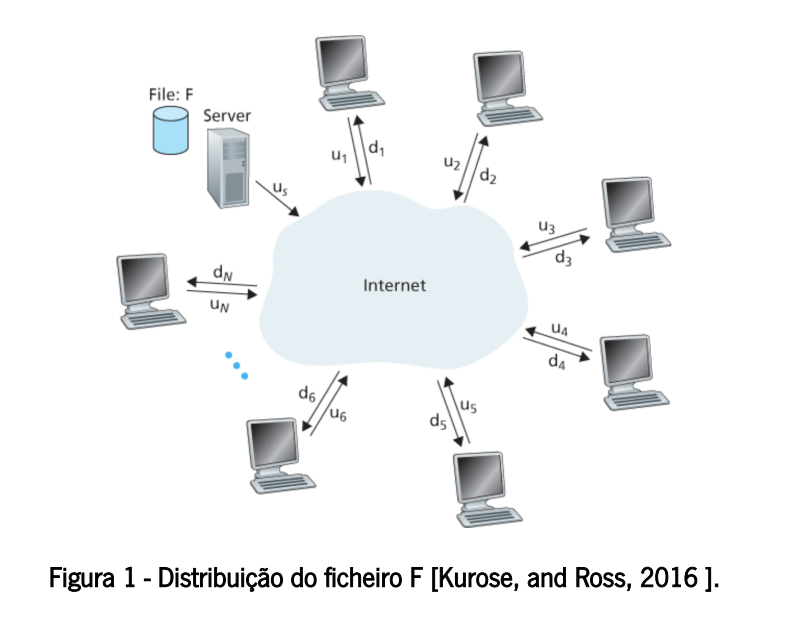
\includegraphics[width=0.4\textwidth]{images/figura1.png}
     \caption{Figura 1}
     \label{fig:my_label}
 \end{figure}
 
\textbf{Sabendo que o servidor tem um débito de upload us=1Gbps, e que di
=100Mbps, calcule, justificando, o tempo mínimo de
distribuição de F pelos N nodos quando N=10, N=100 e N=1000, e para débitos de upload ui de: a) 1Mbps; b) 5Mbps e
c) 10Mbps, usando os modelos de distribuição: (i) cliente-servidor e (ii) peer-to-peer.
Apresente os resultados numa tabela comparativa, bem como o processo de cálculo. Que conclusões pode tirar?}

\vspace{0.5cm}

Pretendemos obter o tempo minimo de distribuição de F pelos N nodos,para N = 10, N = 100 e N = 1000 e débitos de upload $u_i$ de 1Mbps, 5Mbps e 10Mbps.

Para isso, necessitamos de efetuar os cálculos a partir das fórmulas seguintes:
\\

\begin{itemize}
    \item \textbf{Client-Server:}
    \\
    
    
$D_{c-s} \geq max\{NF/u_s,F/d_{min}\}$\\

Onde N varia desde 10, 100 ou 1000, F obtem-se a partir do seguinte cálculo, $F = IDGrupo/10$, $u_s$ calcula-se através do seguinte cálculo, $u_s = 1 * 1000^3$ e o $F/d_{min}$ calcula-se através da seguinte conta $F/(100 * 1000^2)$.

    \item \textbf{Peer-to-Peer:}
    \\
    
    $D_{P2P} \geq max\{F/u_s,F/d_{min},NF/(u_s,+U)\}$\\

Onde N varia desde 10, 100 ou 1000, F obtem-se a partir do seguinte cálculo, $F = IDGrupo/10$, $u_s$ calcula-se através do seguinte cálculo, $u_s = 1000^3$, $F/d_{min}$ calcula-se através da seguinte conta $F/(100 * 1000^2)$ e o $U$ calcula-se através do seguinte cálculo, $U = p * 1000^2$, sendo p o valor do débito de upload que varia desde 1MBps, 5Mbps ou 10Mbps.
\end{itemize}


Para auxiliar no cálculo, criamos um pequeno script que já efetua o cálculo todo, tendo apenas como resultado o tempo.

Nas imagens abaixo, apresentamos o nosso script e os resultados obtidos.

\begin{figure}[h!]
    \centering
    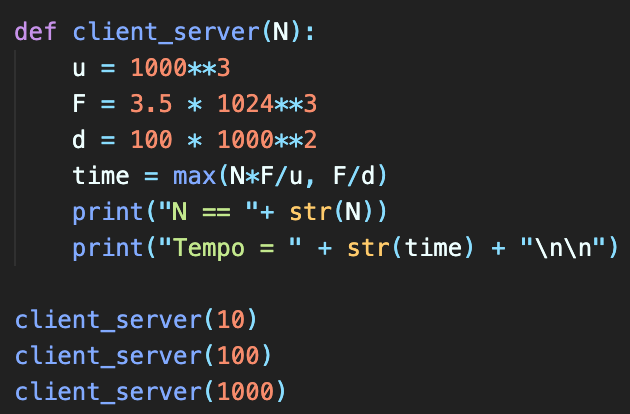
\includegraphics[height=0.3\textwidth, width=0.4\linewidth]{images/C-S.png}
    \caption {Client-Server}
\end{figure}

\begin{figure}[h!]
    \centering
    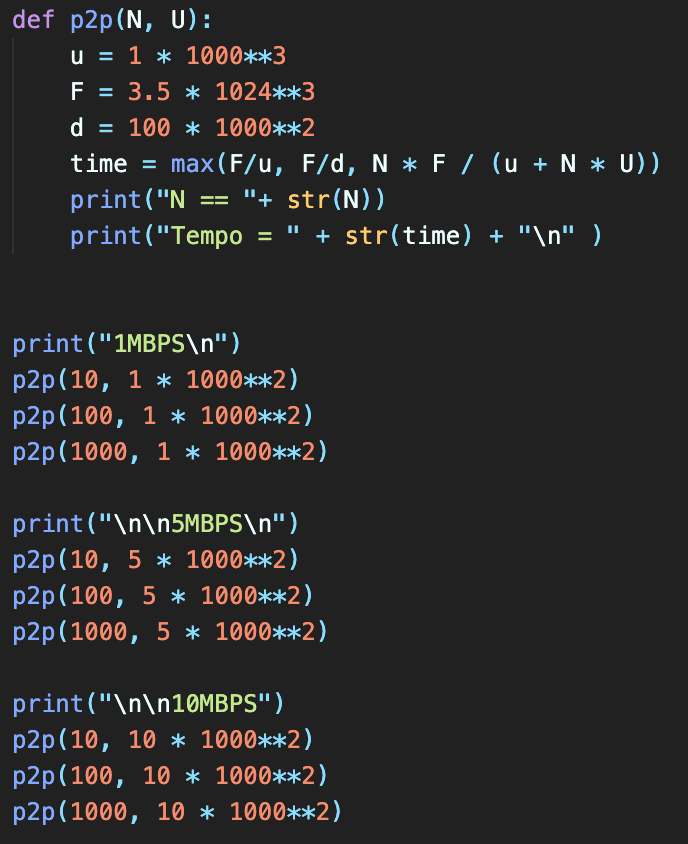
\includegraphics[height=0.45\textwidth, width=0.6\linewidth]{images/P2P.png}
    \caption {Peer-to-Peer}
\end{figure}
\clearpage
\begin{figure}[h!]
    \centering
    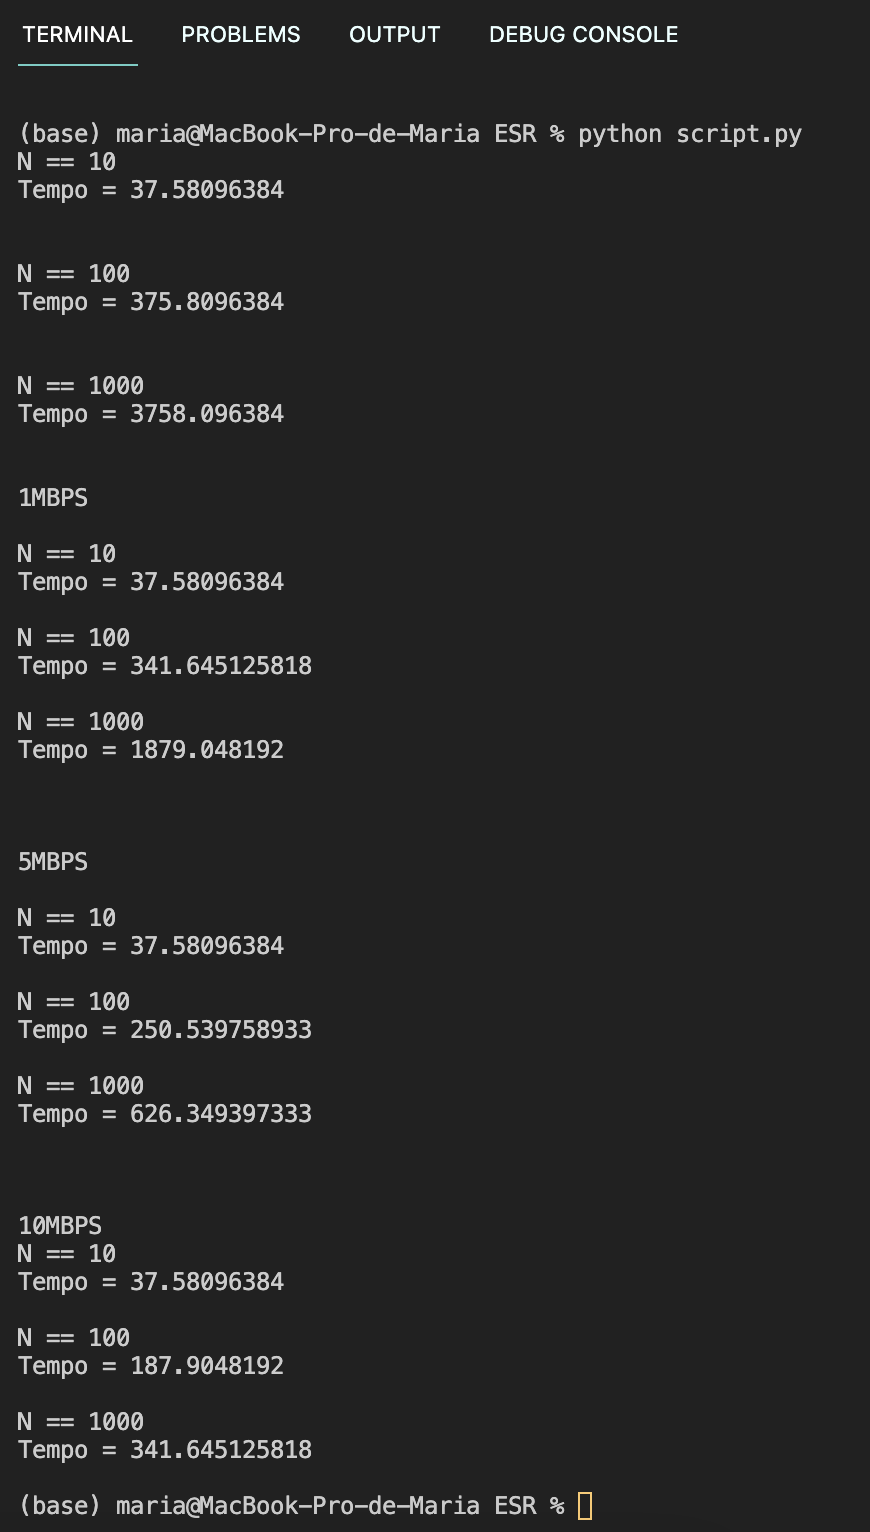
\includegraphics[height=0.8\textwidth, width=0.6\linewidth]{images/Terminal.png}
    \caption {Peer-to-Peer}
\end{figure}

Na tabela abaixo, temos estes valores organizados.
\begin{table}[hbt!]
\center{
\begin{tabular}{|c|c|c|c|}

\hline
\rowcolor[HTML]{DAE8FC} 
\textbf{Modelos\textbackslash{}Nodos} & \textbf{10} & \textbf{100} & \textbf{1000} \\ \hline
\rowcolor[HTML]{ECF4FF} 
\textbf{Client-Server} & 37.581 & 375.810 & 3758.096 \\ \hline
\rowcolor[HTML]{DAE8FC} 
\textbf{Peer-to-Peer 1Mbps} & 37.581 & 341.645 & 1879.048 \\ \hline
\rowcolor[HTML]{ECF4FF} 
\textbf{Peer-to-Peer 5Mbps} & 37.581 & 250.540 & 626.350 \\ \hline
\rowcolor[HTML]{DAE8FC} 
\textbf{Peer-to-Peer 10Mbps} & 37.581 & 187.905 & 341.645 \\ \hline
\end{tabular}
\caption{Resultados}
}
\end{table}

Analisando a tabela, podemos verificar que quando o número de nodos é igual a 10, não há mudança no tempo minimo de distribuição. Assim, concluimos que utilizando estas duas distribuições, quando o número de nodos é reduzido, não evidenciamos diferenças no tempo gasto.
Contudo, conseguimos concluir que a distribuição peer-to-peer é mais rápida e eficiente do que Client-Server, dado que comparado os valores obtidos entre Client-Server com Peer-to-Peer, é na segunda distribuição que. obtemos os menores.
Conseguimos ainda concluir que quanto maior o débito de upload mais eficiente se torna o processo.

\clearpage

\section {Conclusões}

Ao longo deste relatório, abordamos os dois paradigmas \textbf{Client-Server} e \textbf{Peer-to-Peer}. Apresentamos o método do funcionamento de ambos e as suas vantagens e desvantagens. Posteriormente fizemos uma análise de resultados, variando o número de nodos e o débito.\\

Este trabalho prático permitiu-nos aprofundar o conhecimento sobre estes dois paradigmas e perceber onde devereão cada um deles ser utilizados. Para além disso, fez nos conhecer detalhadamente estes dois métodos. Concluimos assim este trabalho de forma positiva, visto que graças a ele aprofundamos o nosso conhecimento sobre redes e os paradigmas nela envolvidos.
\clearpage

\begin{thebibliography}{}

% pergunta 1
\bibitem{1_a}
\url{https://techdifferences.com/difference-between-client-server-and-peer-to-peer-network.html}

\bibitem{1_b1}
\url{https://www.itrelease.com/2021/05/advantages-and-disadvantages-of-client-server-network/}

\bibitem{1_b2}
\url{https://www.jigsawacademy.com/blogs/cyber-security/what-is-client-server-architecture/}

\bibitem{1_b3}
\url{https://www.hitechwhizz.com/2020/11/7-advantages-and-disadvantages-drawbacks-benefits-of-p2p-network.html}

\bibitem{1_b4}
\url{https://www.thecrazyprogrammer.com/2021/03/client-server-architecture.html}

\bibitem{1_b5}
\url{https://www.omnisci.com/technical-glossary/client-server}

\bibitem{1_b6}
\url{https://www.cs.dartmouth.edu/~campbell/cs60/p2p-examples.pdf}

\bibitem{1_b7}
\url{https://digitalthinkerhelp.com/what-is-peer-to-peer-p2p-network-wih-architecture-types-examples/}

% pergunta 2
\bibitem{broadband_speed_guide}
\url{https://www.fcc.gov/consumers/guides/broadband-speed-guide}

\bibitem{network_latency}
\url{https://ecfsapi.fcc.gov/file/6520222942.pdf}

\bibitem{etsi_tr}
\url{https://www.etsi.org/deliver/etsi_tr/102400_102499/102479/01.01.01_60/tr_102479v010101p.pdf}

\end{thebibliography}

\end{document}
